\chapter[Elliptic Curves and $L$-functions]{Elliptic Curves, Galois Representations, and $L$-functions}

This chapter is about elliptic curves and the central role they play
in algebraic number theory.  Our approach will be less systematic and
more a survey than most of the rest of this book.  The goal is to
give you a glimpse of the forefront of research by assuming many basic
facts that can be found in other books (see, e.g.,
\cite{silverman:aec}).

\section{Groups Attached to Elliptic Curves}


\begin{definition}[Elliptic Curve]\label{defn:ec}
  An \defn{elliptic curve} over a field~$K$ is a genus one curve~$E$
  defined over~$K$ equipped with a distinguished point $\O \in E(K)$.
  Here $E(K)$ is the set of all points on $E$ defined over $K$.
\end{definition}
We will not define \emph{genus} in this book, except to note that a
nonsingular curve over~$K$ has genus one if and only if over~$\Kbar$
it can be realized as a nonsingular plane cubic curve.\footnote{
	For a detailed and technical explanation of genus
	see \cite[Ch II.8]{hartshorne} or
	\cite[Ch 7.3]{liu2006algebraic}
}
Moreover, one
can show (using the Riemann-Roch formula) that over any field a genus
one curve with a rational point can always be defined by a projective
cubic equation of the form
$$
  Y^2 Z + a_1 XYZ + a_3 YZ^2  = X^3  + a_2 X^2Z + a_4 XZ^2 + a_6 Z^3.
$$
In this form the distinguished point $\O$ is $(X:Y:Z) = (0:1:0)$.
Note that $\O$ is the only point on the curve with $Z=0$. So we
can consider the rest of the curve in the affine coordinates
by projecting onto the affine plane defined by $Z\neq 0$.
This gives the equation
\begin{equation}\label{weq}
  y^2 +a_1 xy + a_3 y = x^3 + a_2 x^2 + a_4 x + a_6.
\end{equation}
Thus one often presents an elliptic curve by giving a {\em Weierstrass
  equation} (\ref{weq}), though there are significant computational
advantages to other equations for curves (e.g., Edwards coordinates --
see work of Bernstein and Lange in \cite{bernstein2007inverted}).

Using \sage we plot an elliptic curve over the finite field
$\F_7$ and an elliptic curve curve defined over $\Q$.
\begin{sagecode} %skip
\begin{sagecell}
E = EllipticCurve(GF(7), [1,0])
E
\end{sagecell}
\begin{sageout}
Elliptic Curve defined by y^2 = x^3 + x over
    Finite Field of size 7
\end{sageout}
\end{sagecode}
\begin{sagecode}
\begin{sagecell}
E.plot(pointsize=60, gridlines=True)
\end{sagecell}
\begin{sageout}[escapechar=!]
!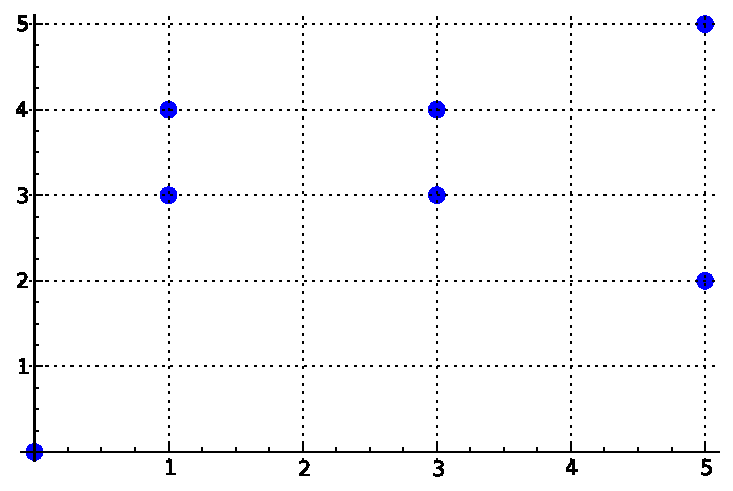
\includegraphics[width=0.9\textwidth]{graphics/ecmod7}
\end{sageout}
\end{sagecode}

\begin{sagecode} %skip
\begin{sagecell}
E = EllipticCurve([1,0])
E
\end{sagecell}
\begin{sageout}
Elliptic Curve defined by y^2 = x^3 + x over
    Rational Field
\end{sageout}
\end{sagecode}
\begin{sagecode}
\begin{sagecell}
E.plot()
\end{sagecell}
\begin{sageout}[escapechar=!]
!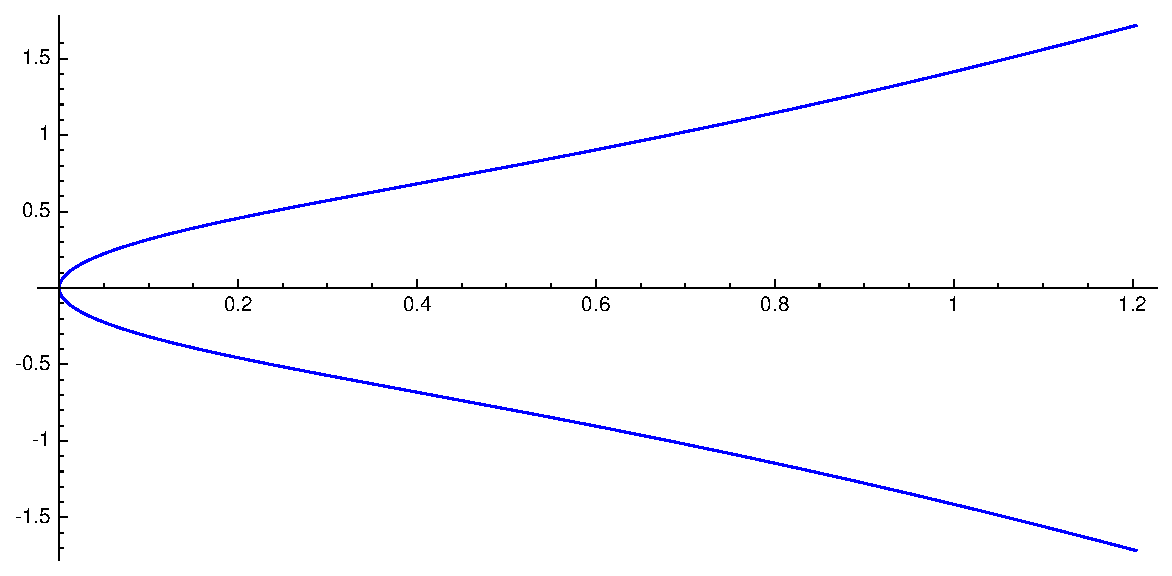
\includegraphics[width=0.9\textwidth]{graphics/ecq}
\end{sageout}
\end{sagecode}

Note that both plots above are of the affine equation $y^2 = x^3 + x$,
and do not include the distinguished point $\O$, which lies at
infinity.

\begin{remark}
The command {\tt{EllipticCurve}} in \sage
can take as input a list {\tt{[a4,a6]}}
of coefficients and returns an elliptic curve given
by a Weirstrass equation with $a_1=a_2=a_3=0$ and
$a_4,a_6$ as specified.
\end{remark}

\subsection{Abelian Groups Attached to Elliptic Curves}
If $E$ is an elliptic curve over~$K$, then we give the set
$E(K)$ of all $K$-rational points on~$E$ the structure of abelian
group with identity element~$\O$.\footnote{
As a reminder, we will not give rigorous proofs of any facts in
this section. For a more detailed and technical explanation of
the group structure for elliptic curves
see \cite[Ch.~III.2]{silverman:aec}.
}
If we embed $E$ in the projective
plane, then this group is determined by the condition that three
points sum to the zero element $\O$ if and only if they lie on a
common line (some care needs to be taken when the points are not
distinct). In our affine picture, a line will intersect the point
at infinity if it is vertical, or equivalently if it of the form
$x=a$ for some fixed $a\in K$.


\begin{example}\label{ex:ecgplaw}
On the curve $y^2=x^3-5x+4$, we have $(0,2) + (1,0) = (3,4)$.
This is because $(0,2)$, $(1,0)$, and $(3,-4)$ are on a common line
(given by the equation $y = 2 - 2x$) hence they sum to zero:
$$
  (0,2) + (1,0) + (3,-4) = \O.
$$
Notice $(3,4)$, $(3,-4)$, and $\O$ (the point at infinity on the curve) are also
on a common line (given by $x = 3$), so $(3,4)=-(3,-4)$.
We can illustration this in \sage:
\begin{sagecode}
\begin{sagecell}
E = EllipticCurve([-5,4])
E(0,2) + E(1,0)
\end{sagecell}
\begin{sageout}
(3 : 4 : 1)
\end{sageout}
\end{sagecode}
\begin{sagecode}
\begin{sagecell} %skip

G = E.plot()
G += points ([(0,2) , (1,0) , (3,4) , (3,-4)],
    pointsize=90 , color='red', zorder=10)
G += line ([(-1,4) , (4,-6)] , color='black')
G += line ([(3,-6) , (3,6)] , color='black')
G.show()
\end{sagecell}
\begin{sageout}[escapechar=!] %skip
!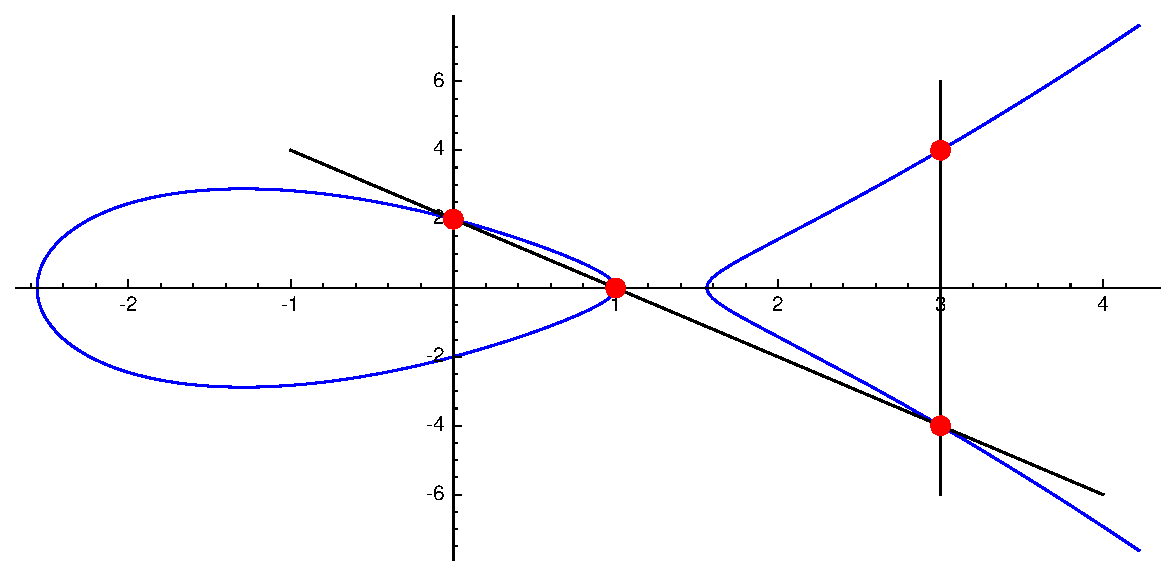
\includegraphics[width=0.925\textwidth]{graphics/grouplaw}
\end{sageout}
\end{sagecode} %link

\noindent
Iterating the group operation often leads quickly to
very complicated points:

\begin{sagecode} %link
\begin{sagecell}
7*E(0,2)
\end{sagecell}
\begin{sageout}
(14100601873051200/48437552041038241 :
-17087004418706677845235922/10660394576906522772066289 :
 1)
\end{sageout}
\end{sagecode}
\end{example}

\begin{remark}
In the previous example we saw that iterating the
group operation led to points which used a lot of digits
to write down. This notion can be made formal and is called
the \emph{height} of the point. The height function is used
to prove the general Mordell-Weil theorem, see
\cite[Ch. VIII.4]{silverman:aec}
\end{remark}

\begin{exercise}\label{ex:ec2torsion}
	Let $E$ be an elliptic curve given by a
	Weirstrass equation such as (\ref{weq}).
	Show that the points of order two are exactly
	the points on $E$ with $y$-coordinate equal to
	$0$.

	\begin{hint}
		Recall that a point $P$ has order $2$ if
		$P + P + \O = \O$, which means the tangent line
		at $P$ goes through the point at infinity.
	\end{hint}
\end{exercise}

That the above condition---three points on a line sum to
zero---defines an abelian group structure on $E(K)$ is not obvious.
Depending on your perspective, the trickiest part is seeing that the
operation satisfies the associative axiom.  The best way to understand
the group operation on $E(K)$ is to view $E(K)$ as being related to a
class group.  As a first observation, note that the ring
$$
 R = K[x,y]/(y^2 +a_1 xy + a_3 y - (x^3 + a_2 x^2 + a_4 x + a_6))
$$
is a Dedekind domain, so $\Cl(R)$ is defined, and every nonzero
fractional ideal can be written uniquely in terms of prime ideals.
When $K$ is a perfect field, the prime ideals correspond to the Galois
orbits of affine points of $E(\overline{K})$.
Note that these do not include the point at infinity.

Let $\Div(E/K)$ be the free abelian group on the Galois orbits of
points of~$E(\overline{K})$, which as explained above is analogous to
the group of fractional ideals of a number field (here we {\em do}
include the point at infinity).
We call the elements of $\Div(E/K)$
{\em divisors}.  Let $\Pic(E/K)$ be the quotient of $\Div(E/K)$ by the
\emph{principal divisors}, i.e., the divisors associated to rational functions
$f\in K(E)^*$ via
$$
 f \mapsto (f) = \sum_{P} \ord_P(f) [P].
$$
Here $K(E)$ is the fraction field of the ring $R$ defined above.
Note that the principal divisor associated to $f$ is analogous to the
principal fractional ideal associated to a nonzero element of a number
field.  The definition of $\ord_P(f)$ is analogous to the ``power
of~$P$ that divides the principal ideal generated by~$f$''.
%TODO reference text for this? Hartshorne abstract non-singular curves
%TODO or somewhere in Silverman Ch VIII? or an algebra text on
%TODO valuations? or an exercise?
Define the \emph{class group} $\Pic(E/K)$ to be the quotient of the
divisors by the principal divisors, so we have
an exact sequence:
$$
  1\to K(E)^*/K^* \to \Div(E/K) \to \Pic(E/K) \to 0.
$$
%TODO is the 1 - ... - 0 weird?

A key difference between elliptic curves and algebraic number fields
is that the principal divisors in the context of elliptic curves all
have degree~$0$, i.e., the sum of the coefficients of the
divisor~$(f)$ is always~$0$.  This might be a familiar fact to you:
the number of zeros of a nonzero rational function on a projective
curve equals the number of poles, counted with multiplicity.  If we
let $\Div^0(E/K)$ denote the subgroup of divisors of degree~$0$, then
we have an exact sequence
$$
  1\to K(E)^*/K^* \to \Div^0(E/K) \to \Pic^0(E/K) \to 0.
$$

To connect this with the group law on $E(K)$, note that there
is a natural map
$$
 E(K) \to \Pic^0(E/K), \qquad P \mapsto [P-\O].
$$
Using the Riemann-Roch theorem, one can prove that this map
is a bijection, which is moreover an isomorphism of abelian groups.
Thus really when we discuss the group of $K$-rational
points on an $E$, we are talking
about the class group $\Pic^0(E/K)$.

Recall that we proved (Theorem~\ref{thm:finiteclassgrp}) that the
class group $\Cl(\O_K)$ of a number field is finite.
The  group $\Pic^0(E/K) =E(K)$ of an elliptic curve can be
either finite (e.g., for $y^2 + y = x^3 - x + 1$) or infinite (e.g.,
for $y^2 + y = x^3 - x$), and determining which is the case for any particular
curve is one of the central unsolved problems in number theory.

The Mordell-Weil theorem (see Chapter~\ref{ch:weakmw}) asserts that if $E$ is
an elliptic curve over a number field $K$, then there is a nonnegative integer
$r$, referred to as the \emph{algebraic rank of $E$}, such that
\begin{equation}\label{eqn:mw}
  E(\Q) \ncisom \Z^r \oplus T,
\end{equation}
where $T$ is a finite group.   This is similar to Dirichlet's unit theorem, which
gives the structure of the unit group of the ring of integers of a number field.
The main difference is that $T$ need not be cyclic, and computing $r$ appears to be
much more difficult than just finding the number of real and complex roots of
a polynomial!

\begin{example}
\sage has algorithms which can compute this rank for us.
For example we can compute the ranks of the curves
$y^2 + y = x^3 - x + 1$ and $y^2 + y = x^3 - x$ respectively.
\begin{sagecode}
\begin{sagecell}
EllipticCurve([0,0,1,-1,1]).rank()
\end{sagecell}
\begin{sageout}
0
\end{sageout}
\begin{sagecell}
EllipticCurve([0,0,1,-1,0]).rank()
\end{sagecell}
\begin{sageout}
1
\end{sageout}
\end{sagecode}
\end{example}

Also, if $L/K$ is an arbitrary extension of fields, and $E$ is an
elliptic curve over~$K$, then there is a natural inclusion
homomorphism $E(K)\hra E(L)$.  Thus instead of just obtaining one group
attached to an elliptic curve, we obtain a whole collection, one for
each extension of~$L$.  Even more generally, if $S/K$ is an arbitrary
scheme, then $E(S)$ is a group, and the association $S\mapsto E(S)$
defines a functor from the category of schemes to the category of
groups.  Thus each elliptic curve gives rise to map:
$$
 \left\{\text{Schemes over $K$}\right\} \longrightarrow
\left\{\text{Abelian Groups}\right\}
$$

\begin{remark}
	Elliptic curves are not the only objects that induce
	a functor from schemes to groups.
	\emph{Abelian varieties} are a larger class of
	schemes, which includes elliptic curves,
    that also induce such a functor.
    For more on Abelian varieties see
    \cite{milne:abvars}.
\end{remark}

\subsection{A Formula for Adding Points}

We close this section with an explicit formula for
adding two points in $E(K)$.
If $E$ is an elliptic curve over a field $K$,
given by an equation $y^2=x^3+ax+b$, then we
can compute the group addition using the following
algorithm.
\begin{algorithm}[Elliptic Curve Group Law]\label{alg:grouplaw}
Given $P_1, P_2\in E(K)$,
this algorithm computes the sum $R=P_1+P_2 \in E(K)$.
{\sf \begin{enumerate}
\item{}[One Point $\O$] If $P_1=\O$ set $R=P_2$ or if $P_2=\O$ set $R=P_1$
and terminate.  Otherwise write $P_i=(x_i,y_i)$.
\item{}[Negatives]  If $x_1 = x_2$ and $y_1 = -y_2$, set $R=\O$ and terminate.
\item{}[Compute $\lambda$]\label{alg:grouplaw_3}
Set $\ds \lambda = \begin{cases}
 (3x_1^2+a)/(2y_1) & \text{if }P_1 = P_2,\\
(y_1-y_2)/(x_1-x_2) & \text{otherwise.}
\end{cases}$\\
Note: If $y_1=0$ and $P_1=P_2$, output $\O$ and terminate.
\item{}[Compute Sum]\label{alg:grouplaw_4}  Then
$R = \ds \left(\lambda^2 -x_1 - x_2, -\lambda x_3 - \nu\right)$,
where $\nu = y_1 - \lambda x_1$ and~$x_3$ is the~$x$ coordinate of $R$.
\end{enumerate}}
\end{algorithm}

\subsection{Other Groups}
There are other abelian groups attached to elliptic curves, such as
the torsion subgroup $E(K)_{\tor}$ of elements of $E(K)$ of finite
order.  The torsion subgroup is (isomorphic to) the group $T$ that
appeared in Equation~\eqref{eqn:mw} above).  When $K$ is a number
field, there is a group called the Shafarevich-Tate group $\Sha(E/K)$
attached to~$E$, which plays a role similar to that of the class group
of a number field (though it is an open problem to prove that
$\Sha(E/K)$ is finite in general).  The  definition of $\Sha(E/K)$ involves Galois
cohomology, so we wait until Chapter~\ref{ch:gc} to define it.  There
are also component groups attached to~$E$, one for each prime of
$\O_K$.  These groups all come together in the Birch and
Swinnerton-Dyer conjecture (see \url{http://wstein.org/books/bsd/}).

%TODO change this reference please
%TODO is there another book on bsd?

\section[Galois Representations]{Galois Representations Attached to Elliptic Curves}

Let~$E$ be an elliptic curve over a number field~$K$.
In this section we attach representations of
$G_K = \Gal(\Kbar/K)$ to~$E$, and use them to define an $L$-function
$L(E,s)$.   This $L$-function is yet another generalization of the
Riemann Zeta function, that is different from the $L$-functions
attached to complex representations $\Gal(\Qbar/\Q)\to \GL_n(\C)$,
which we encountered before in Section~\ref{sec:artin}.

There is a natural action of $G_K$ on the points of $E(\overline{K})$.
Given a point $P=(a,b)\in E(\overline{K})$ we define $\sigma(P)$ to be
the point $(\sigma(a),\sigma(b))$. Since~$E$ is defined over~$K$ the
point~$\sigma(P)$ will again lie on~$E$ so the action is well
defined. Note that the group structure on~$E$ is defined by
algebraic formulas with coefficients in~$K$. It follows that the
action commutes with point addition meaning that
$\sigma(P+Q) = \sigma(P)+\sigma(Q)$. Now fix an integer $n$.
From what we have seen, the subgroup
$$
E[n] = \{P \in E(\Kbar) : nP = \O\}
$$
is invariant under the action of $G_K$.
We thus obtain a homomorphism
$$
\rhobar_{E,n} : G_K \to \Aut(E[n]).
$$

\begin{warning}
Though the action of $G_K$ leaves the group $E[n]$ fixed,
it may act non-trivially on individual elements! Otherwise
$\rhobar_{E,n}$ would not be very interesting.
\end{warning}

For any positive integer~$n$, the group $E[n]$ is isomorphic as an
abstract abelian group to $(\Z/n\Z)^2$.  There are various
related ways to see why this is true. One is to use the Weierstrass
$\wp$-theory to parametrize $E(\C)$ by the the complex numbers, i.e.,
to find an isomorphism $\C/\Lambda \isom E(\C)$, where $\Lambda$ is a
lattice in $\C$ and the isomorphism is given by $z\mapsto
(\wp(z),\wp'(z))$ with respect to an appropriate choice of coordinates
on $E(\C)$.  It is then an easy exercise to verify that
$(\C/\Lambda)[n]\isom (\Z/n\Z)^2$.
For a detailed and rigorous walk through of this method see
\cite[Ch.~1.4]{diamond-shurman}.

Another way to understand $E[n]$ is to use the fact
that $E(\C)_{\tor}$ is isomorphic
to the quotient
$$\H_1(E(\C),\Q)/\H_1(E(\C),\Z)$$
of homology groups and that the homology of a curve
of genus~$g$ is isomorphic to $\Z^{2g}$.
Then we have a non-canonical isomorphism
$$
 E[n]\approx (\Q/\Z)^2[n] = (\Z/n\Z)^2.
$$

Technically the previous arguments have shown $E(\C)[n] \approx (\Z/n\Z)^2$.
However, our definition of $E[n]$ used points in $E(\overline{K})$.
So we need to show the points $E(\C)[n]$ are actually defined over
$\overline{K}$. Note that $E(\C)[n]$ is finite and invariant under
$\Aut(\C/\overline{K})$ for the same reason as $E[n]$ was invariant under
$\Gal(\overline{K}/K)$ (point addition is defined by algebraic formulas with
coefficients in $K$). It follows that $E(\C)[n]$ is indeed defined over 
$E(\overline{K})$ so the arguments above show that
$E[n] \approx \left(\Z/n\Z\right)^2$.

\begin{remark}
	Notice that the arguments above used many analytic facts about
	geometry over $\C$ (e.g. homology, analytic structure) in order to
	prove algebraic facts (e.g. the number of torsion points) about
	$E(\overline{K})$. This is part of a more general concept denoted
	\emph{Lefschetz principle} which generally relates geometry over an
	algebraically closed field of characteristic $0$ to geometry over
	$\C$. For more on this see \cite[Ch.~VI.6]{silverman:aec}.
\end{remark}

\begin{exercise}\label{QE[p]finitegaloisext}
	Let $E$ be an elliptic curve defined over a number
	field~$K$. Fix an integer $n$ and consider the
	extension of $K$ given by
	$$
	K(E[n]) = K(\{a,b : (a,b) \in E[n]\}).
	$$
	Show that $K(E[n])/K$ is a finite Galois extension.
	
	Hint: By the arguments above $\#E[n] = n^2$ which shows
	the extension is finite. Next recall that $E[n]$ is left
	invariant by the action of $\Gal(\overline{K}/K)$. What
	can you say about the embeddings from $K(E[n])$ into
	$\overline{K}$ which leave $K$ fixed?
\end{exercise}

\begin{example}
Consider the case when $n=2$. From Exercise~\ref{ex:ec2torsion}
we know that the points in $E[2]$ are exactly the points with
$y$-coordinate $0$. Let $E$ be the elliptic curve given by
$E: y^2 = x^3 + x + 1$. If $y=0$ then $x$ has to be a root
of the polynomial $x^3 + x + 1$, so the points in $E[2]$
are defined over the splitting field of $x^3 + x + 1$.
We can compute these points in \sage.

\begin{sagecode}
\begin{sagecell}
E = EllipticCurve([1,1]); E
\end{sagecell}
\begin{sageout}
Elliptic Curve defined by y^2 = x^3 + x + 1 over
    Rational Field
\end{sageout}
\begin{sagecell}
R.<x> = QQ[]; R
\end{sagecell}
\begin{sageout}
Univariate Polynomial Ring in x over Rational Field
\end{sageout}
\end{sagecode} %link
\begin{sagecode} %link
\begin{sagecell}
f = x^3 + x + 1
K.<a> = NumberField(f)
M.<b> = K.galois_closure(); M
\end{sagecell}
\begin{sageout}
Number Field in b with defining polynomial
    x^6 + 6*x^4 + 9*x^2 + 31
\end{sageout}
\end{sagecode} %link
\begin{sagecode} %link
\begin{sagecell}
F = E.change_ring(M)
T = F.torsion_subgroup(); T
\end{sagecell}
\begin{sageout}
Torsion Subgroup isomorphic to Z/2 + Z/2 associated
    to the Elliptic Curve defined by y^2 = x^3 + x + 1
    over Number Field in b with defining polynomial
    x^6 + 6*x^4 + 9*x^2 + 31
\end{sageout}
\end{sagecode} %link
\begin{sagecode} %link
\begin{sagecell}
T.gens()
\end{sagecell}
\begin{sageout}
((1/18*b^4 + 5/18*b^2 + 1/2*b + 2/9 : 0 : 1),
    (1/18*b^4 + 5/18*b^2 - 1/2*b + 2/9 : 0 : 1))
\end{sageout}
\end{sagecode}
\noindent
Note that this matches with what we expected: we computed
two generators for $E[2]$ (the output of the last cell)
corresponding to two generators of $\left(\ZZ/2\ZZ\right)^2$.

\end{example}

If $n=p$ is a prime, then upon chosing a basis for the two-dimensional
$\F_p$-vector space $E[p]$, we obtain an isomorphism $\Aut(E[p]) \isom
\GL_2(\F_p)$.  We thus obtain a mod~$p$ Galois representation
$$
 \rhobar_{E,p} : G_K \to \GL_2(\F_p).
$$
This representation $\rhobar_{E,p}$ is continuous if $\GL_2(\F_p)$ is endowed with the
discrete topology, because the field $K(E[p])$
is a Galois extension of~$K$ of finite degree
by Exercise~\ref{QE[p]finitegaloisext}.

In order to attach an $L$-function to $E$, one could try to embed
$\GL_2(\F_p)$ into $\GL_2(\C)$ and use the construction of Artin
$L$-functions from Section~\ref{sec:artin}.
Unfortunately, this approach is doomed in general, since
$\GL_2(\F_p)$ frequently does not embed in $\GL_2(\C)$.
The following Sage session shows that for $p=5,7$, there are
no 2-dimensional irreducible representations of $\GL_2(\F_p)$,
so $\GL_2(\F_p)$ does not embed in $\GL_2(\C)$.
The notation in the output below is
{\tt [degree of rep, number of times it occurs]}.
\begin{sagecode}
\begin{sagecell}
GL(2,GF(2)).gap().CharacterTable().CharacterDegrees()
\end{sagecell}
\begin{sageout}
[ [ 1, 2 ], [ 2, 1 ] ]
\end{sageout}
\begin{sagecell}
GL(2,GF(3)).gap().CharacterTable().CharacterDegrees()
\end{sagecell}
\begin{sageout}
[ [ 1, 2 ], [ 2, 3 ], [ 3, 2 ], [ 4, 1 ] ]
\end{sageout}
\begin{sagecell}
GL(2,GF(5)).gap().CharacterTable().CharacterDegrees()
\end{sagecell}
\begin{sageout}
[ [ 1, 4 ], [ 4, 10 ], [ 5, 4 ], [ 6, 6 ] ]
\end{sageout}
\begin{sagecell}
GL(2,GF(7)).gap().CharacterTable().CharacterDegrees()
\end{sagecell}
\begin{sageout}
[ [ 1, 6 ], [ 6, 21 ], [ 7, 6 ], [ 8, 15 ] ]
\end{sageout}
\end{sagecode}

Instead of using the complex numbers, we use the
\emph{$p$-adic numbers}\footnote{
For a review of $p$-adic numbers and $p$-adic analysis
see \cite{koblitz1996p}.
}, as
follows.  For each power $p^m$ of $p$, we have defined a homomorphism
$$
  \rhobar_{E,p^m}: G_K \to \Aut(E[p^m]) \ncisom \GL_2(\Z/p^m\Z).
$$
We combine together all of these representations (for all $m\geq 1$)
using the inverse limit.
Recall that the $p$-adic numbers are
$$
  \Z_p = \varprojlim \Z/p^m\Z,
$$
which is the set of all compatible choices of integers modulo $p^m$ for
all $m$.
We obtain a (continuous) homomorphism
$$
  \rho_{E,p}: G_K \to \Aut(\varprojlim E[p^m]) \isom \GL_2(\Z_p),
$$
where $\Z_p$ is the ring of $p$-adic integers.  The composition of
this homomorphism with the reduction map $\GL_2(\Z_p) \to \GL_2(\F_p)$
is the representation $\rhobar_{E,p}$, which we defined above, which
is why we denoted it by $\rhobar_{E,p}$. We
next try to mimic the construction of $L(\rho,s)$ from
Section~\ref{sec:artin} in the context of a $p$-adic Galois
representation $\rho_{E,p}$.

\begin{definition}[Tate module]
The \emph{$p$-adic Tate module of $E$} is
$$
  T_p(E) = \varprojlim E[p^n].
$$
\end{definition}

Let $M$ be the fixed field of $\ker(\rho_{E,p})$. The image of
$\rho_{E,p}$ is infinite, so $M$ is an infinite extension of~$K$.
Fortunately, one can prove that~$M$ is ramified at only finitely many
primes (the primes of \emph{bad reduction} for $E$ and $p$---see
\cite{serre-tate}).
If~$\ell$ is a prime of $K$, let $D_{\ell}$ be a choice of
decomposition group for
some prime~$\p$ of~$M$ lying over~$\ell$, and let $I_{\ell}$ be the
inertia group.  We haven't defined inertia and decomposition groups
for infinite Galois extensions, but the definitions are almost the
same: choose a prime of $\O_M$ over~$\ell$, and let $D_{\ell}$ be the
subgroup of $\Gal(M/K)$ that leaves~$\p$ invariant.  Then the
submodule $T_p(E)^{I_{\ell}}$ of inertia invariants is a module for
$D_{\ell}$ and the characteristic polynomial $F_{\ell}(x)$ of
$\Frob_{\ell}$ on $T_p(E)^{I_{\ell}}$ is well defined (since inertia
acts trivially).  Let $R_{\ell}(x)$ be the polynomial obtained by
reversing the coefficients of $F_{\ell}(x)$.  One can prove that
$R_{\ell}(x) \in \Z[x]$ and that $R_{\ell}(x)$, for $\ell\neq p$ does
not depend on the choice of~$p$.  Define $R_{\ell}(x)$ for $\ell=p$
using a different prime $q\neq p$, so the definition of $R_{\ell}(x)$
does not depend on the choice of~$p$.
\begin{definition}
The $L$-series of $E$ is
$$
 L(E,s) = \prod_{\ell} \frac{1}{R_\ell(\ell^{-s})}.
$$
\end{definition}

A prime~$\p$ of $\O_K$ is a prime of \emph{good reduction} for~$E$ if
there is an equation for $E$ such that $E \mod \p$ is an elliptic
curve over the field $\O_K/\p$. If $K=\Q$ and $\ell$ is a prime of
good reduction for~$E$, then one can show that that
$R_{\ell}(\ell^{-s}) = 1 - a_\ell \ell^{-s} + \ell^{1-2s},$
where
$
  a_{\ell} = \ell + 1 - \#\tilde{E}(\F_\ell)
$
and $\tilde{E}$ is the reduction of a local minimal
model for~$E$ modulo~$\ell$.  (There is a similar statement
for $K\neq \Q$.)

One can prove using fairly general techniques that the product
expression for $L(E,s)$ defines a holomorphic function in some right
half plane of~$\C$, i.e., the product converges for all~$s$ with
$\Re(s)>\alpha$, for some real number~$\alpha$.

Recall that the Artin $L$-function from Section~\ref{sec:artin}
(see Equation~\ref{eqn:artin}) extended to meromorphic function
on the entire complex plane and we conjectured that the $L$-function
of any continuous representation of $\Gal(\Qbar/\Q) \to \GL_n(\C)$ also
extends to a meromorphic function on $\C$. We could ask the same
question for the $L$-functions attached to elliptic curves. However,
we will instead ask for something stronger:
\begin{center}
\emph{Does the $L$-function $L(E,s)$ attached to an
elliptic curve $E$ extends to a holomorphic function on $\C$?}
\end{center}
This question was one of the central topics
in number theory in the late 1990s and early 2000s.
An amazing fact is that the question has been answered
in the affirmative.
\begin{theorem}\label{conj:holo}
The function $L(E,s)$ extends to a holomorphic
function on all~$\C$.
\end{theorem}
This is a corollary to the modularity theorem described
in the next section, see Corollary~\ref{cor:hecke}.


\subsection{Modularity of Elliptic Curves over $\Q$}
Fix an elliptic curve $E$ over~$\Q$.  In this section we will explain
what it means for $E$ to be modular, and note the connection with
Conjecture~\ref{conj:holo} from the previous section.

First, we give the general definition of modular form (of weight~$2$).
The complex {\em upper half plane} is
$
  \h  = \{z  \in \C : \Im(z) > 0\}.
$
A {\em cuspidal modular form} $f$ of level~$N$ (of weight~$2$) is a holomorphic
function
$
   f : \h \to \C
$
such that $\lim_{z\to i\infty} f(z) = 0$ and for every integer matrix
$\abcd{a}{b}{c}{d}$ with determinant~$1$ and $c\equiv 0 \pmod{N}$, we have
$$
  f\left( \frac{az + b}{cz + d} \right)
         = (cz+d)^{-2} f(z).
$$

For each prime number $\ell$ of good reduction, let $a_\ell = \ell+1 -
\#\tilde{E}(\Fell)$.  If $\ell$ is a prime of bad reduction let
$a_\ell = 0,1,-1$, depending on how singular the reduction~$\tilde{E}$
of~$E$ is over $\Fell$.  If $\tilde{E}$ has a cusp, then $a_\ell=0$,
and $a_\ell=1$ or $-1$ if $\tilde{E}$ has a node; in particular,
let $a_\ell=1$ if
and only if the tangents at the cusp are defined over~$\Fell$.

Extend the definition of the $a_\ell$ to $a_n$ for all positive
integers~$n$ as follows.  If $\gcd(n,m)=1$ let $a_{nm} = a_n \cdot
a_m$.  If $p^r$ is a power of a prime~$p$ of good reduction, let
$$
 a_{p^r} = a_{p^{r-1}}\cdot a_p \,\,-\,\, p \cdot a_{p^{r-2}}.
$$
If $p$ is a prime of bad reduction let $a_{p^r} = (a_p)^r$.

Attach to $E$ the function
$$
  f_E(z) = \sum_{n=1}^{\infty} a_n e^{2\pi i z}.
$$
It is an extremely deep theorem that $f_E(z)$ is actually
a cuspidal modular form, and not just some random function.


The following theorem is called the modularity theorem for elliptic
curves over~$\Q$.  Before it was proved it was known as the
Taniyama-Shimura-Weil conjecture.
\begin{theorem}[Wiles, Brueil, Conrad, Diamond, Taylor]
Every elliptic curve over $\Q$ is modular, i.e, the function
$f_E(z)$  is a cuspidal modular form.
\end{theorem}

\begin{corollary}[Hecke]\label{cor:hecke}
  If $E$ is an elliptic curve over~$\Q$, then the $L$-function
  $L(E,s)$ has an analytic continuous to the whole complex plane.
%and
%  satisfies a functional equation (symmetry) that relates $L(E,s)$ to
%  $L(E,2-s)$.
\end{corollary}
%TODO some explanation/background for this?



%%% Local Variables:
%%% mode: latex
%%% TeX-master: "ant"
%%% End: